\documentclass[../master]{subfiles}

%\graphicspath{{../eps/}}

\begin{document}

\chapter{シミュレーション}
\label{chap::simulation}
\section{$\alpha$線源を用いた測定}
\ref{sec::detection_gas_candidate}節で考えた各ガスについて,
シミュレーションの基準となるトラックを測定した.
また,それらのデータから各ガスにおけるドリフトスピード,ガス増幅率,トラックの幅を測定した.
測定には${}^{241}{\rm Am}$の$\alpha$線源を用いた.
図\ref{fig::a_source_track}に$\alpha$線源のトラックの一例を示す.
図\ref{fig::a_source_track}では検出ガスに\isoButaneHydro を用いた.
\ref{sec::detection_gas_candidate}節では6種類の候補を考えたが,
ここからは単体のiso-$\rm C_{4}H_{10}$を除いた5種類について考えていく.
これはディフュージョン係数が大きくトラックが太くなると予測されることと,
圧力が\SI{15}{\hecto\pascal}と低く安定したTPC の動作が難しいと予測されるためである.
\begin{figure}
  \centering
  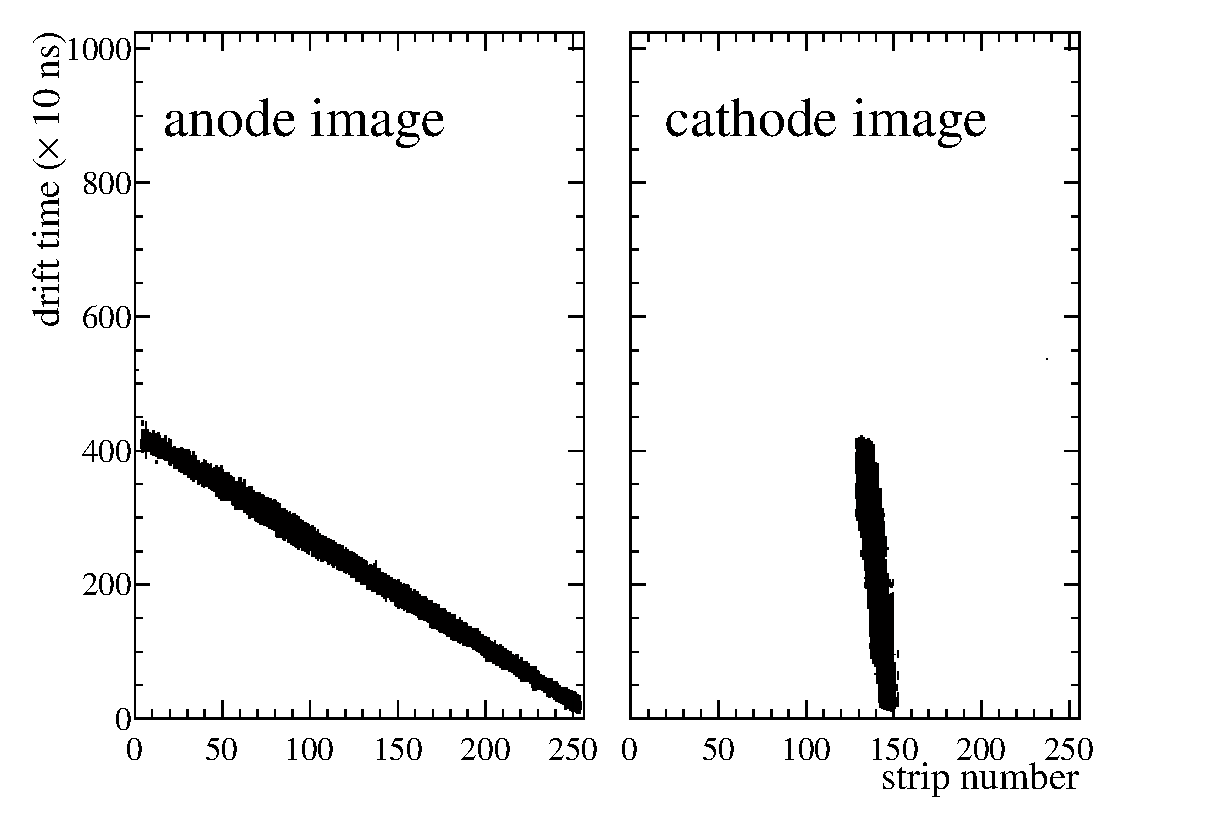
\includegraphics[clip, width=0.9\columnwidth]{0210_7.eps}
  \caption[$\alpha$線源で測定したトラックの一例.]
          {$\alpha$線源で測定したトラックの一例.
          検出ガスは\isoButaneHydro を用いた.}
  \label{fig::a_source_track}
\end{figure}

\subsection{ドリフトスピード}
電子のドリフトスピードを線源によって得られるトラックから求める.
測定には図\ref{pic::alpha_collimator}のような線源コリメータを用いる.
このコリメータはアクリルで作られており,1つの\ang{0},4つの\ang{30}の穴が開いている.
このコリメータを用いることで$\alpha$線を\ang{0}と\ang{30}の方向に限定することができる.
図\ref{fig::drift_v_image}の右のようにドリフト方向に$\Delta y$,それと垂直な方向に$\Delta z$移動するとき,
\begin{equation}
  \Delta y = \tan(\ang{30})\Delta z \label{eq::deltay_deltaz}
\end{equation}
となる.
MAIKo TPC で取得したトラックの横方向の変分を$\Delta strip$,縦方向の変分を$\Delta t$,
ドリフトスピードを$drift\_v$とすると,
\begin{align}
  \frac{\Delta z}{\SI{0.4}{\milli\metre}} & = \Delta strip \label{eq::deltaz}\\
  \frac{\Delta y}{drift\_v} & = \Delta t \label{eq::deltay}
\end{align}
式 (\ref{eq::deltay_deltaz}, \ref{eq::deltaz}, \ref{eq::deltay}) より
\begin{equation}
  drift\_v = \frac{\tan(\ang{30})~\Delta strip\times\SI{0.4}{\milli\metre}}{\Delta t}
\end{equation}
とドリフトスピードが求まる.
\begin{figure}
  \centering
  \begin{subfigure}{0.45\columnwidth}
    \centering
    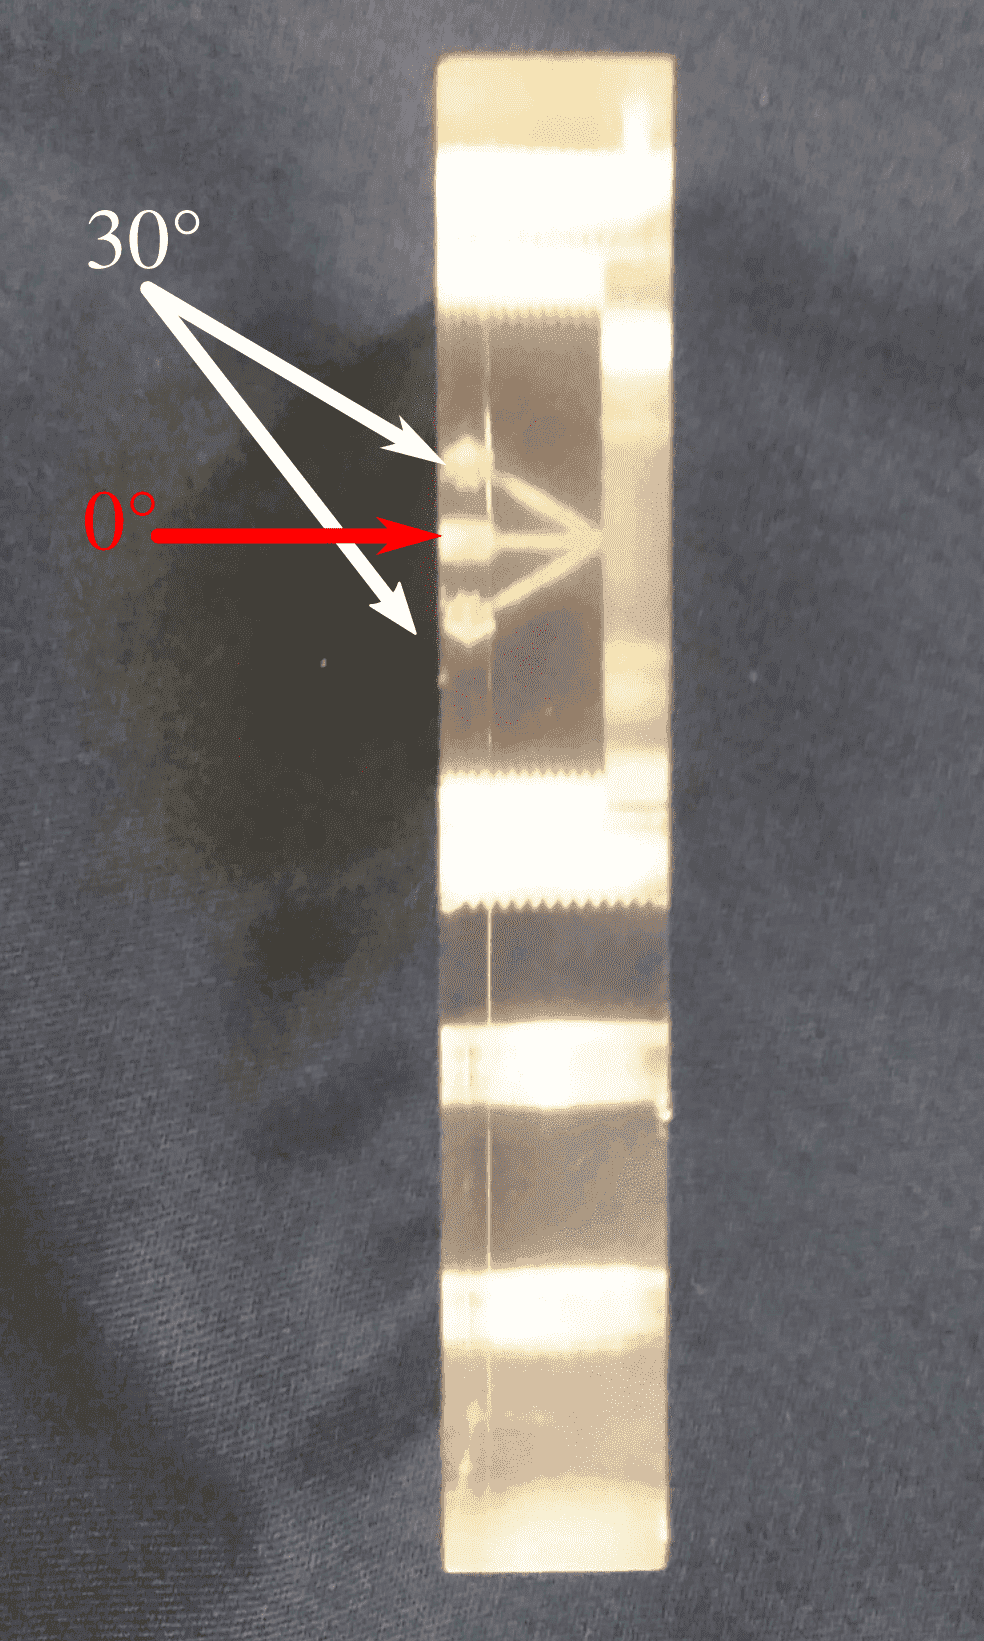
\includegraphics[clip, width=0.8\columnwidth]{image30580-min.png}
    \caption{側面.}
  \end{subfigure}
  \begin{subfigure}{0.45\columnwidth}
    \centering
    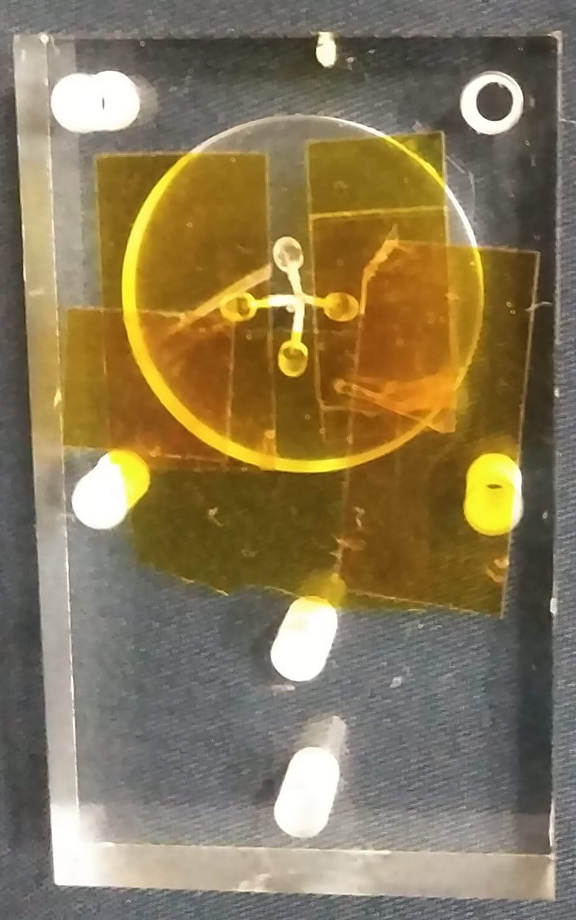
\includegraphics[clip, width=0.8\columnwidth]{IMG_20191225_183542_clip.jpg}
    \caption{正面.}
  \end{subfigure}
  \caption[線源コリメータ.]
          {線源コリメータ.中央に\ang{0},上下左右に\ang{30}の穴が開いている.
            \ang{0}の穴と1つの\ang{30}の穴を除いてカプトンテープで塞ぐことで,
            余計な$\alpha$線が出ないようにしている.
          }
          \label{pic::alpha_collimator}
\end{figure}
\begin{figure}
  \centering
  \begin{minipage}{0.45\columnwidth}
    \centering
    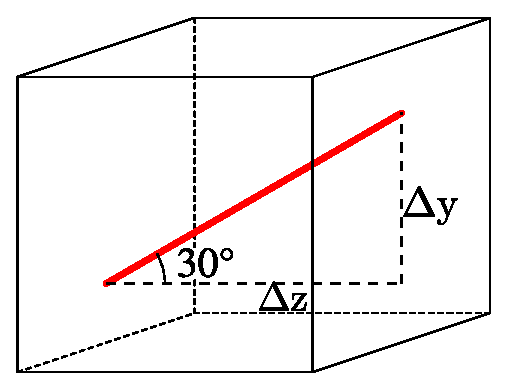
\includegraphics[clip, width=0.9\columnwidth]{drift_v_source.eps}
  \end{minipage}
  \begin{minipage}{0.45\columnwidth}
    \centering
    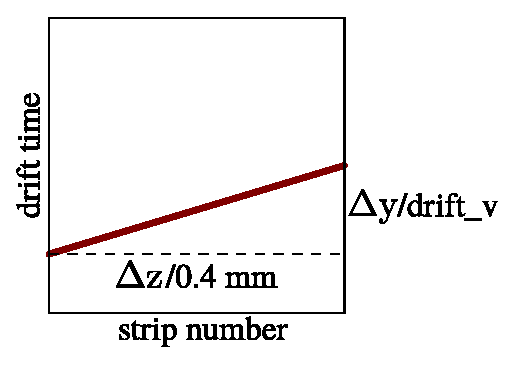
\includegraphics[clip, width=0.9\columnwidth]{drift_v_image.eps}
  \end{minipage}
  \caption[\ang{30}に方向を限定した$\alpha$線と取得される画像データのイメージ.]
          {\ang{30}に方向を限定した$\alpha$線 (左) と取得される画像データ (右) のイメージ.}
  \label{fig::drift_v_image}
\end{figure}

$\alpha$線源を用いて測定したドリフトスピードとMagboltz で求めた値を
表\ref{tab::drift_speed_compare}に示す.
$\alpha$線源を用いて測定したドリフトスピードと Magboltz を用いて計算したドリフトスピードがおおよそ一致していることが分かる.
\Methane は実測とMagboltz とがずれているが,ガスに含まれる水分の影響が考えられる.
\Methane のみ\SI{50}{\hecto\pascal} とその他のガスと比較して圧力が半分であるため,不純物の影響が大きく出ていると考えられる.
\begin{table}
  \centering
  \caption{実測したドリフトスピードとMagboltzで求めたドリフトスピードの比較.}
  \label{tab::drift_speed_compare}
  \begin{tabular}{cccc}
    \toprule
    gas & ドリフト電場 (\si{\volt\per\milli\metre}) & 実測 (\si{\milli\metre\per\nano\second})
    & Magboltz (\si{\milli\metre/\nano\second})\\
    \midrule
    \Methane & 0.429 & 0.0126 & 0.0145 \\
    \MethaneHydro & 4.32 & 0.0140 & 0.0140 \\
    \MethaneHerium & 1.89 & 0.0135 & 0.0140 \\
    \isoButaneHydro & 6.82 & 0.0137 & 0.0140 \\
    \isoButaneHerium & 3.29 & 0.0139 & 0.0141 \\
    \bottomrule
  \end{tabular}
\end{table}
%\begin{figure}
%  \centering
%  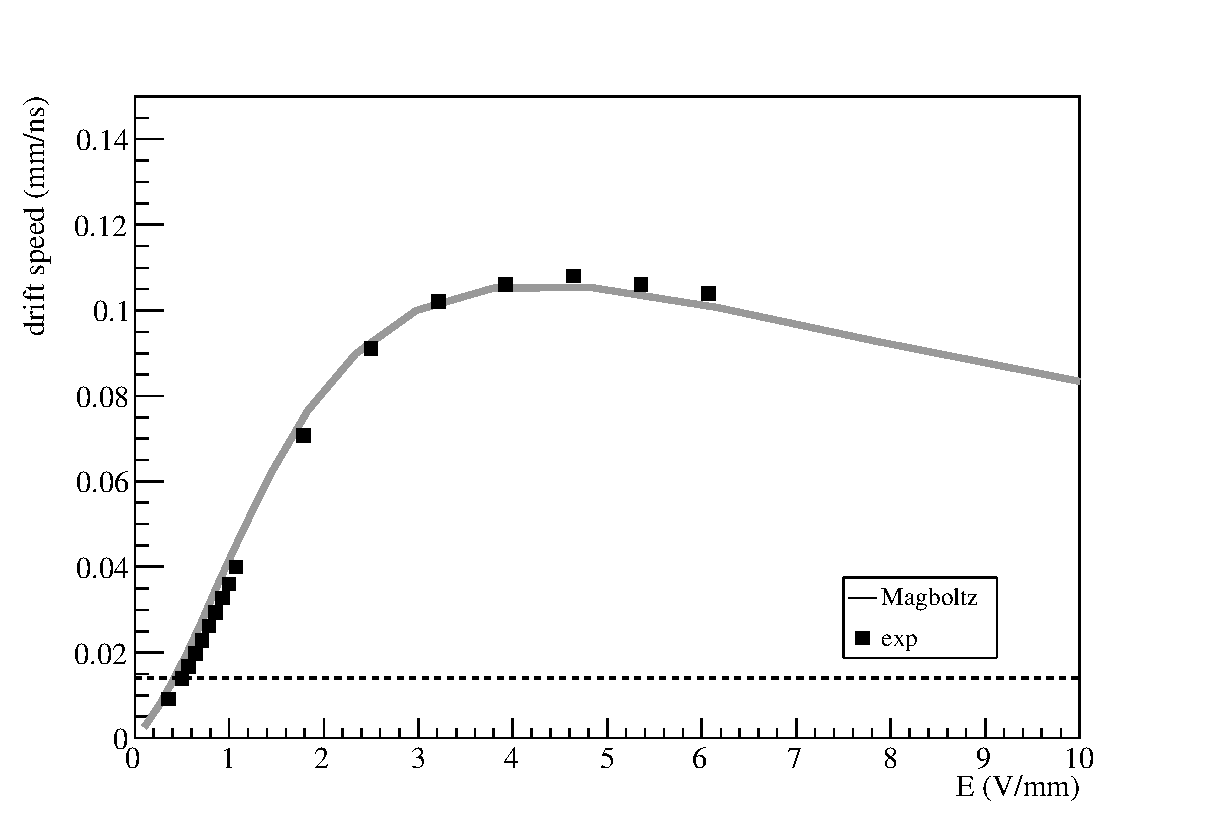
\includegraphics[clip, width=0.9\columnwidth]{drift_v_CH4.eps}
%  \caption[検出ガスに${\rm CH_{4}}$を用いたときのドリフトスピードの電場依存性.]
%          {検出ガスに${\rm CH_{4}}$を用いたときのドリフトスピードの電場依存性.
%            図中の点線は0.014 mm/ns を示す.}
%  \label{fig::drift_v_CH4}
%%  \includegraphics[clip, width=0.7\columnwidth]{drift_v_CH4_H2.eps}
%  \caption{}
%  \label{fig::drift_v_CH4_H2}
%%  \includegraphics[clip, width=0.7\columnwidth]{drift_v_CH4_He.eps}
%  \caption{}
%  \label{fig::drift_v_CH4_He}
%  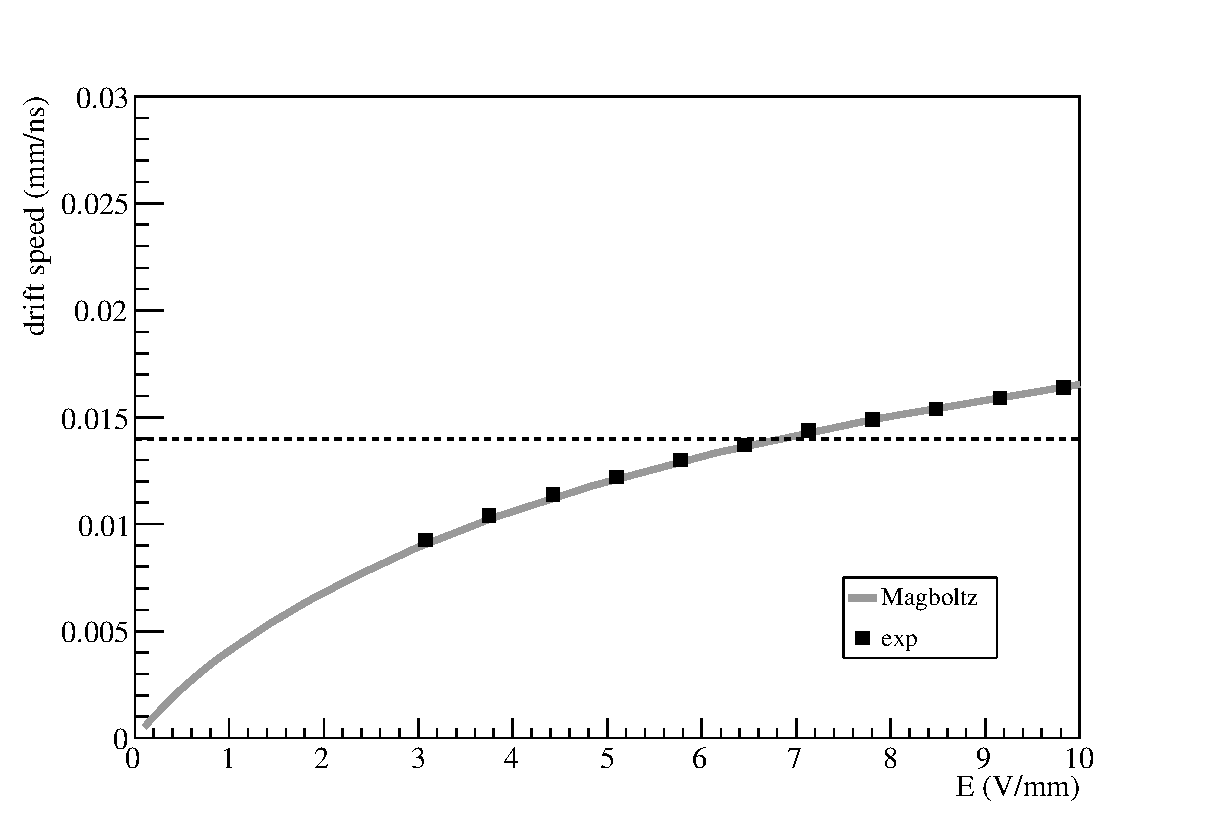
\includegraphics[clip, width=0.9\columnwidth]{drift_v_iC4H10_H2.eps}
%  \caption[検出ガスにiso-${\rm C_{4}H_{10}}$を用いたときのドリフトスピードの電場依存性.]
%          {検出ガスにiso-${\rm C_{4}H_{10}}$を用いたときのドリフトスピードの電場依存性.
%        p    図中の点線は0.014 mm/ns を示す.}
%  \label{fig::drift_v_iC4H10_H2}
%%  \includegraphics[clip, width=0.7\columnwidth]{drift_v_iC4H10_He.eps}
%  \caption{}
%  \label{fig::drift_v_iC4H10_He}
%\end{figure}

\subsection{電子増幅率}
電圧パラメータを変更させたときの増幅率の変化を測定した.
増幅率を計算するためには荷電粒子が検出ガス中を通過した際に発生する電子数 ($N_{\rm e}$) と
増幅後に$\mu$-PICによって収集された電子数 ($N'_{\rm e}$) の比を取る.
$N_{\rm e}$はガス中での荷電粒子のエネルギー損失とガスのW値から求める.
$N'_{\rm e}$は$\mu$-PICで収集した電荷から求める.
詳しい計算方法について以下で述べる.

ガス中で荷電粒子がエネルギーを落とすと,W値あたり平均1個の電子を電離する.
そのため,荷電粒子のエネルギー損失をW値で割ることで$N_{\rm e}$が求まる.
各ガスのエネルギー損失とW値~\cite{energy_per_ion_pair,pdg}を表\ref{tab::energy_loss_and_W_val}に示す.
測定に用いた$\alpha$線源からは平均4.2 MeVの$\alpha$粒子が出ていることが他の測定によりわかっている.
エネルギー損失は\SI{4.2}{\mega\electronvolt}の$\alpha$粒子が$\mu$-PIC 32 strip分の
距離 (\SI{12.8}{\milli\metre}) で落とすエネルギーを示している.
\begin{table}
  \centering
  \caption[検出ガスのW値とエネルギー損失と$N_{\rm e}$.]
          {検出ガスのW値~\cite{energy_per_ion_pair,pdg}とエネルギー損失と$N_{\rm e}$.
          エネルギー損失は荷電粒子がガス中を\SI{12.8}{\milli\metre} 進んだ時のものである.}
  \label{tab::energy_loss_and_W_val}
  \begin{tabular}{cccc}
    \toprule
    gas & W値 (\si{\electronvolt}) & energy loss (\si{\kilo\electronvolt}) & $N_{\rm e}$\\
    \midrule
    \Methane         & 29.1 & 56.5 & 1.94$\times 10^{3}$ \\
    \MethaneHydro    & 34.2 & 53.4 & 1.56$\times 10^{3}$ \\
    \MethaneHerium   & 39.2 & 59.3 & 1.51$\times 10^{3}$ \\
%    iso-${\rm C_{4}H_{10}}$                 & 26.0 & 0.0552 & 2.12$\times 10^{3}$ \\
    \isoButaneHydro  & 35.4 & 62.0 & 1.75$\times 10^{3}$ \\
    \isoButaneHerium & 44.0 & 58.0 & 1.32$\times 10^{3}$ \\
    \bottomrule
  \end{tabular}
\end{table}

$\mu$-PICからの信号波形は32 strips まとめて図\ref{fig::FADC_waveform}のようなFADC 情報として取得している.
この信号波形を時間で積分することによって32 strips で収集した電荷量を計算することができる.
$\mu$-PICで取得した電気信号は読み出し回路内部で800倍に増幅され,
入力インピーダンス\SI{50}{\ohm}で電流値を電圧値に変換して取得している.
よって,式 (\ref{eq::N'e})で求めることができる.
\si{\elementarycharge}は電荷素量である.
\begin{equation}
  N'_{\rm e} = \frac{\int V (t) dt}{ 50 \times 800 \times \si{\elementarycharge}}
  \label{eq::N'e}
\end{equation}
各ガスの増幅率を表\ref{tab::multiplying_rate}に示す.
ここでは,GEMと$\mu$-PIC の両方による増幅率となっている.
\begin{table}
  \centering
  \caption{各ガスの電子増幅率.}
  \label{tab::multiplying_rate}
  \begin{tabular}{cc}
    \toprule
    gas & 増幅率 (倍) \\
    \midrule
    \Methane         & 700 \\
    \MethaneHydro    & 354 \\
    \MethaneHerium   & 322 \\
    \isoButaneHydro  & 272 \\
    \isoButaneHerium & 392 \\
    \bottomrule
  \end{tabular}
\end{table}

\subsection{幅}
本実験の目的である3$\alpha$に崩壊するイベントではトラックが太いと複数のトラックを区別できなくなり,
トラックの抽出を正しくできなくなる.
\ang{0}の$\alpha$粒子によるトラックで幅を測定した.
図\ref{fig::track_width}に示すように,
トラックの幅にはanode strip 128~chのclock方向の幅を用いる.
このようにして決定したトラックの幅を表\ref{tab::track_width},図\ref{fig::diffusion_compare}に示す.
図\ref{fig::diffusion_compare}から分かるようにトラックの幅とディフュージョン係数には相関がある.
ディフュージョン係数,トラックの幅ともに\isoButaneHydro が最も小さいことが分かる.
\begin{figure}
  \centering
  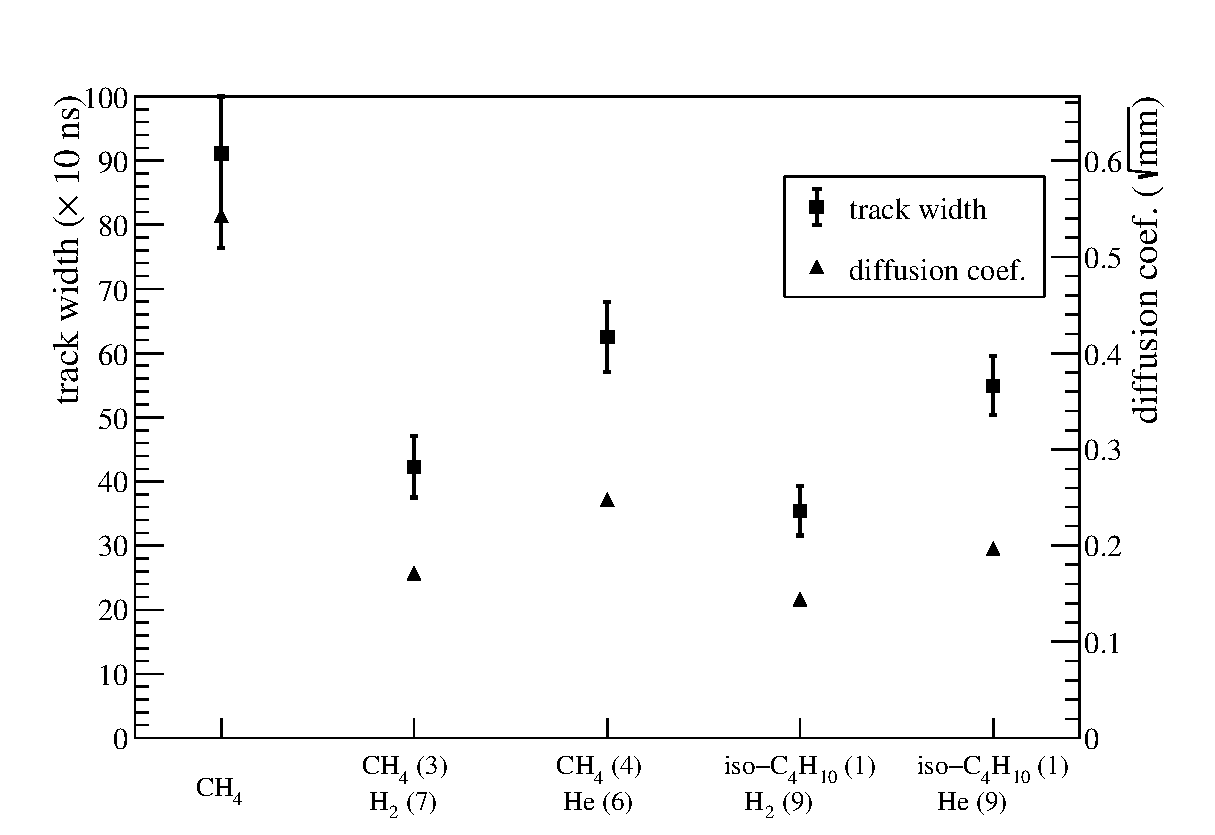
\includegraphics[clip, width=0.5\columnwidth]{track_width.eps}
  \caption{トラックの幅の決定方法のイメージ.
    トラックの幅は有感領域の中央であるanode strip 128~chのclock方向の幅を用いる.}
  \label{fig::track_width}
\end{figure}

\begin{table}
  \centering
  \caption{各ガスのトラックの幅.}
  \label{tab::track_width}
  \begin{tabular}{cc}
    \toprule
    gas & トラックの幅 ($\times \SI{10}{\nano\second}$)\\
    \midrule
    \Methane         & 91.1 \\
    \MethaneHydro    & 42.3 \\
    \MethaneHerium   & 62.5 \\
    \isoButaneHydro  & 35.4 \\
    \isoButaneHerium & 54.9 \\
    \bottomrule
  \end{tabular}
\end{table}

\begin{figure}
  \centering
  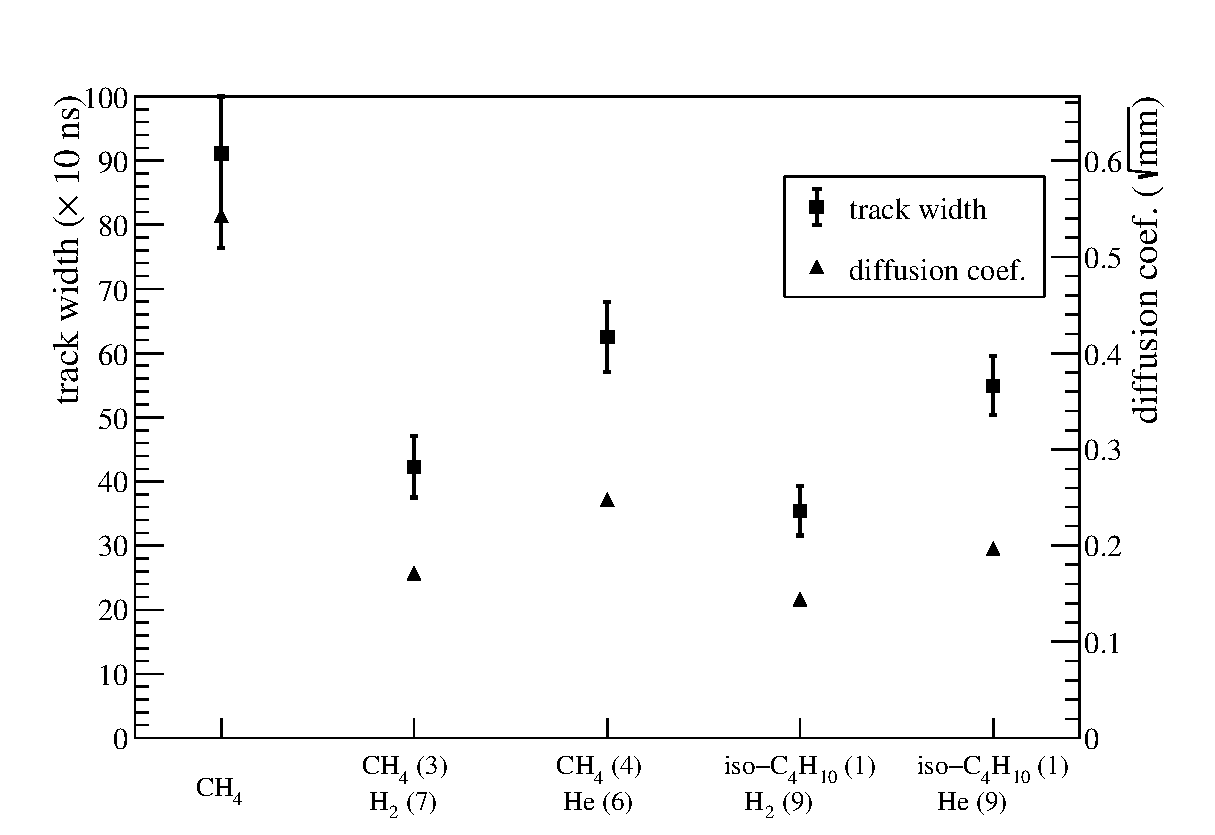
\includegraphics[clip, width=0.9\columnwidth]{diffusion_compare.eps}
  \caption{Magboltz で求めたディフージョン係数とトラックの幅.}
  \label{fig::diffusion_compare}
\end{figure}

\section{シミュレーションによる線源データの再現}
MAIKo TPC から得られるトラックをGarfield++~\cite{garfield++}と
Magboltz~\cite{magboltz}を用いたシミュレーションにより再現した.
シミュレーションでは,ドリフト電場,W値,電子増幅率,検出ガスの密度をfixed parameters,
TOTの閾値をfree parameterとした.
シミュレーションは以下のような手順%(図\ref{fig::simulation_flow})
で行った.
\begin{enumerate}
\item\label{sim::particle_generate}
  トラックを生成する荷電粒子のエネルギー,運動量を決定し,
  Garfield++のSrimTrack に登録する.
\item
  SrimTrack によりトラックの周囲に電子を生成する.
\item
  電子をMagboltz で求めたドリフトスピードで読み出し領域へドリフトさせる.
\item
  読み出し領域に到達した電子1つにつき図\ref{fig::mu-pic_readout}にあるような電気信号を
  各strip の信号波形に追加する.
\item
  設定した閾値により,信号波形をTOTに変換しanode image とcathode image を作る.
\end{enumerate}
TOTの閾値は\SI{0.1}{\milli\volt}とした.
$\alpha$線源を用いた場合のシミュレーションと測定の比較を図\ref{fig::track_comp_ch4},
\ref{fig::track_comp_ch4_h2}, \ref{fig::track_comp_ch4_he}, 
\ref{fig::track_comp_ic4h10_h2}, \ref{fig::track_comp_ic4h10_he}に示す.
それぞれの検出ガスで$\alpha$線源によるトラックを,
シミュレーションで再現できていることが分かる.
\begin{figure}
  \centering
  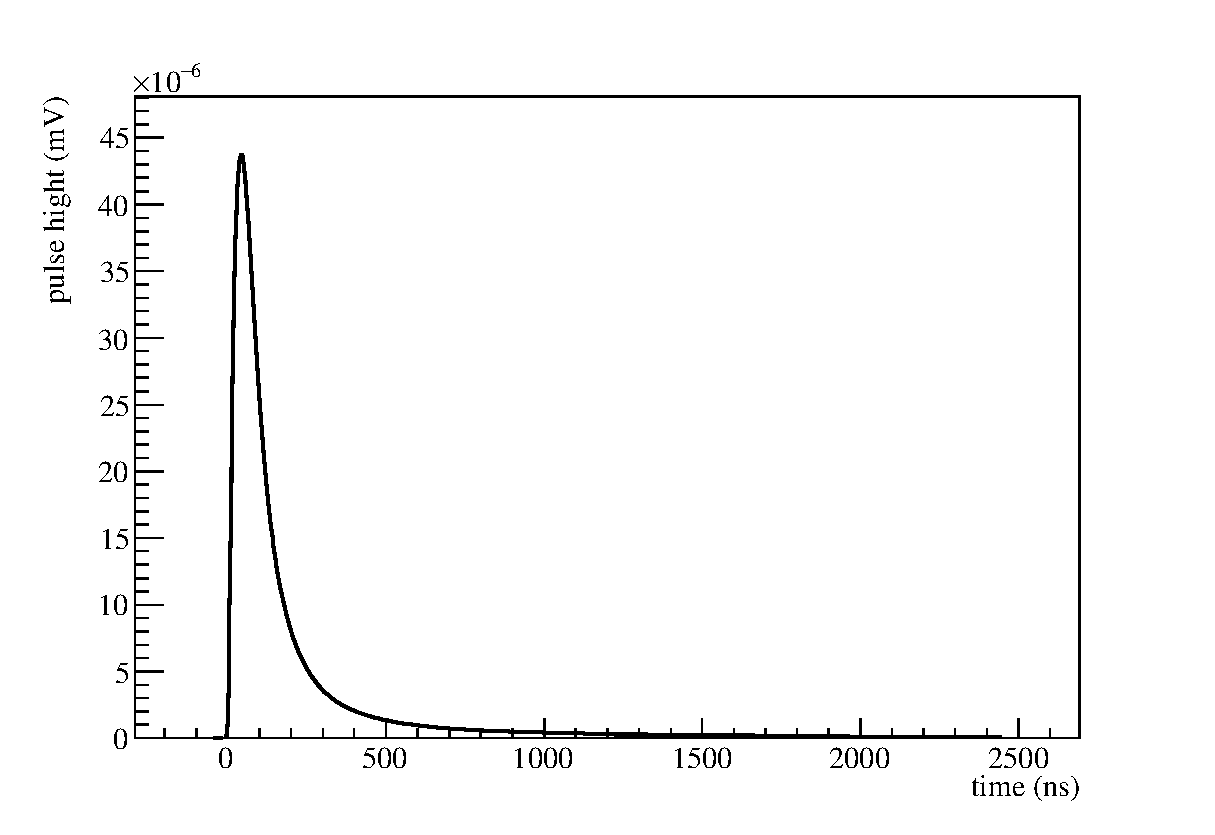
\includegraphics[clip, width=0.9\columnwidth]{waveform.eps}
  \caption{1電子が$\mu$-PICに到達した時に読み出される電気信号.}
  \label{fig::mu-pic_readout}
\end{figure}

\begin{figure}
  \centering
  \begin{subfigure}{0.48\columnwidth}
    \centering
    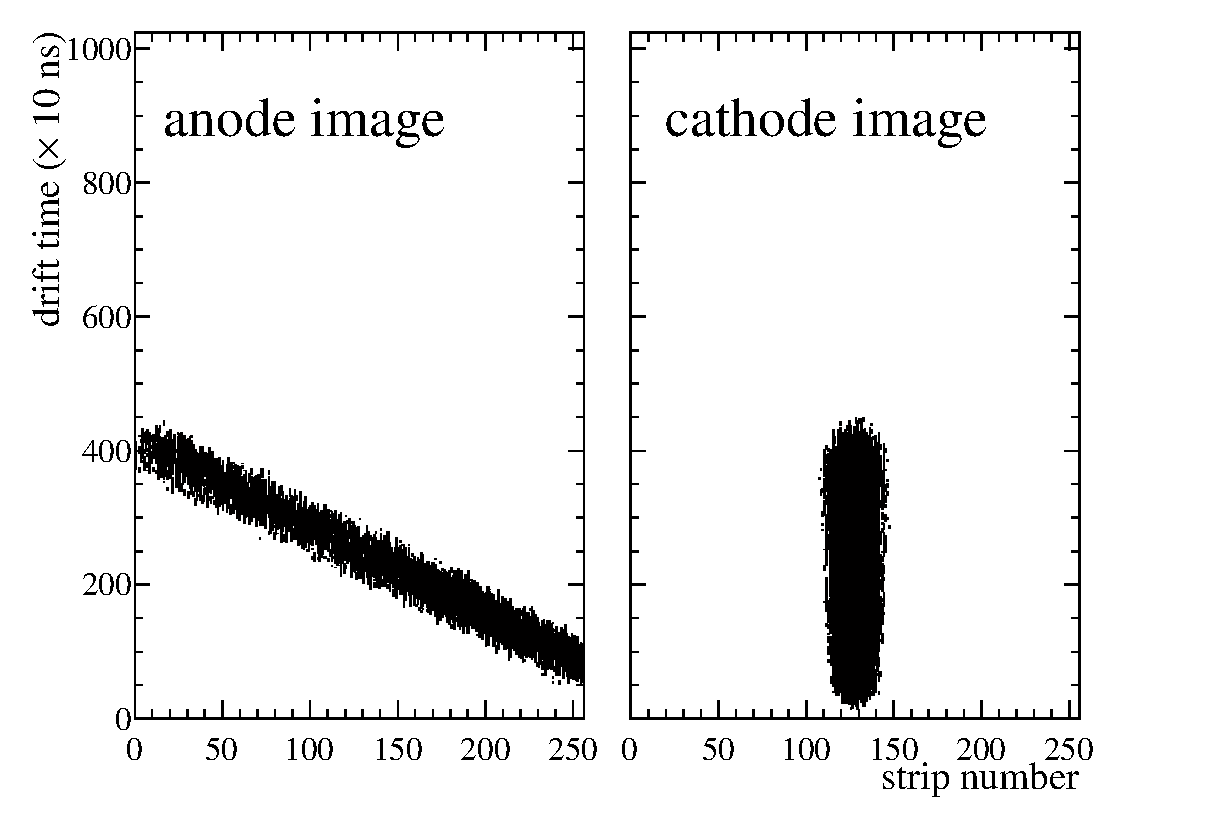
\includegraphics[clip, width=\columnwidth, trim=0 0 50 0]{CH4_0.eps}
    \caption{シミュレーションによるトラック.}
  \end{subfigure}
  \begin{subfigure}{0.48\columnwidth}
    \centering
    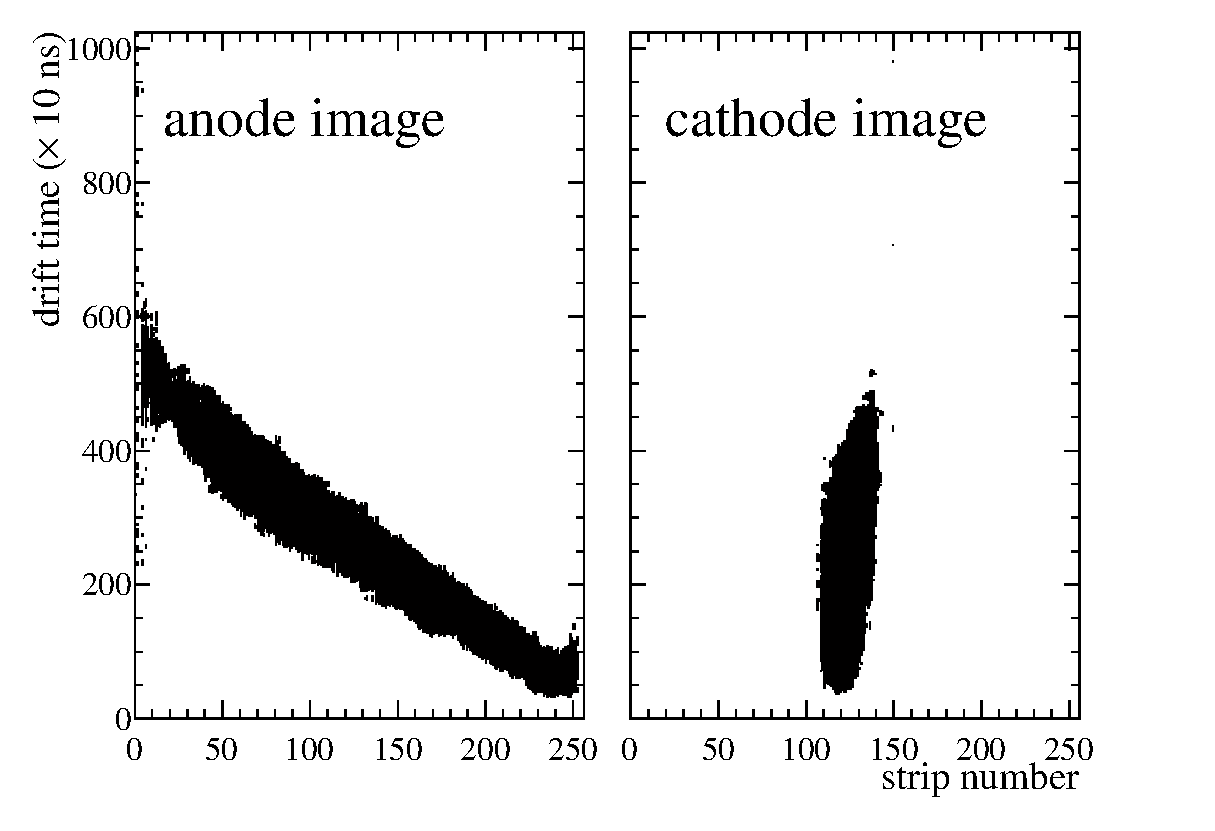
\includegraphics[width=\columnwidth, trim=0 0 50 0]{0160_5.eps}
    \caption{$\alpha$線源によるトラック.}
  \end{subfigure}
  \caption{\Methane の場合.}
  \label{fig::track_comp_ch4}
\end{figure}

\begin{figure}
  \centering
  \begin{subfigure}{0.48\columnwidth}
    \centering
    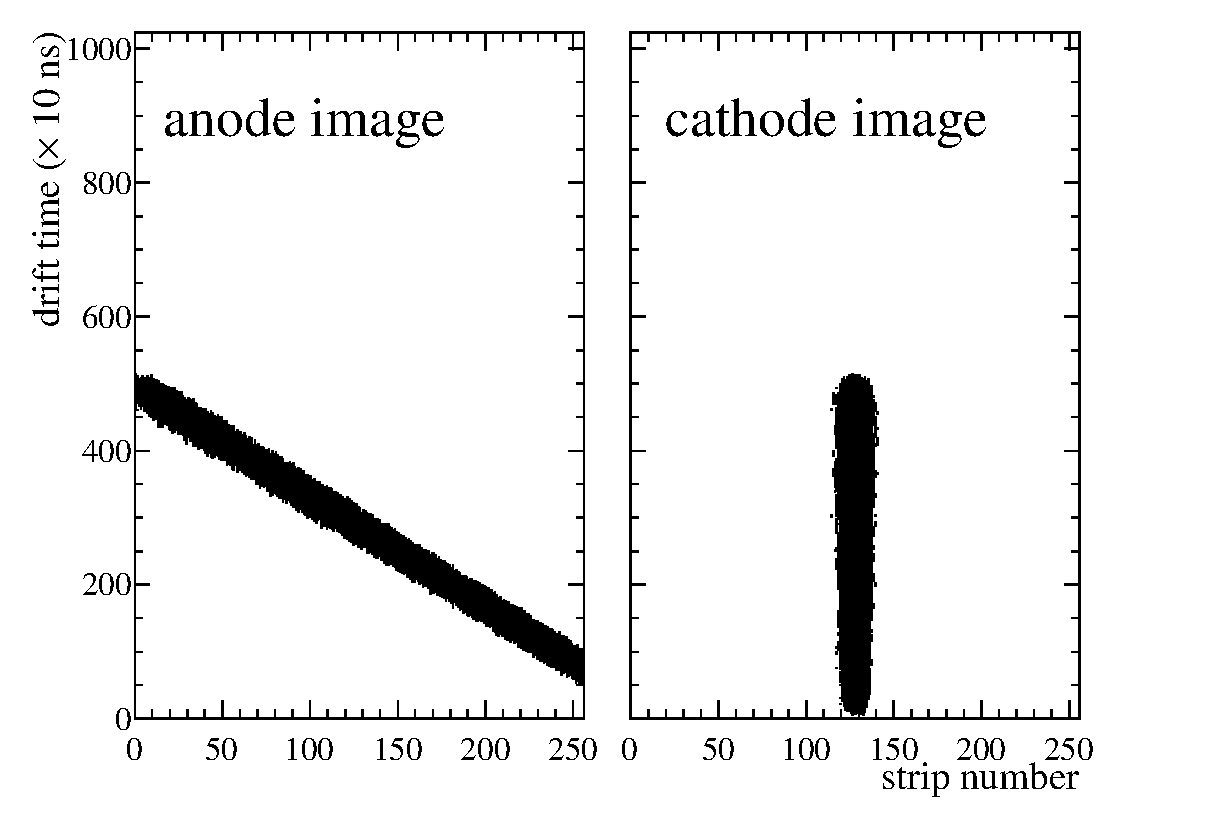
\includegraphics[clip, width=\columnwidth, trim=0 0 50 0]{CH4_3_H2_7_0.eps}
    \caption{シミュレーションによるトラック.}
  \end{subfigure}
  \begin{subfigure}{0.48\columnwidth}
    \centering
    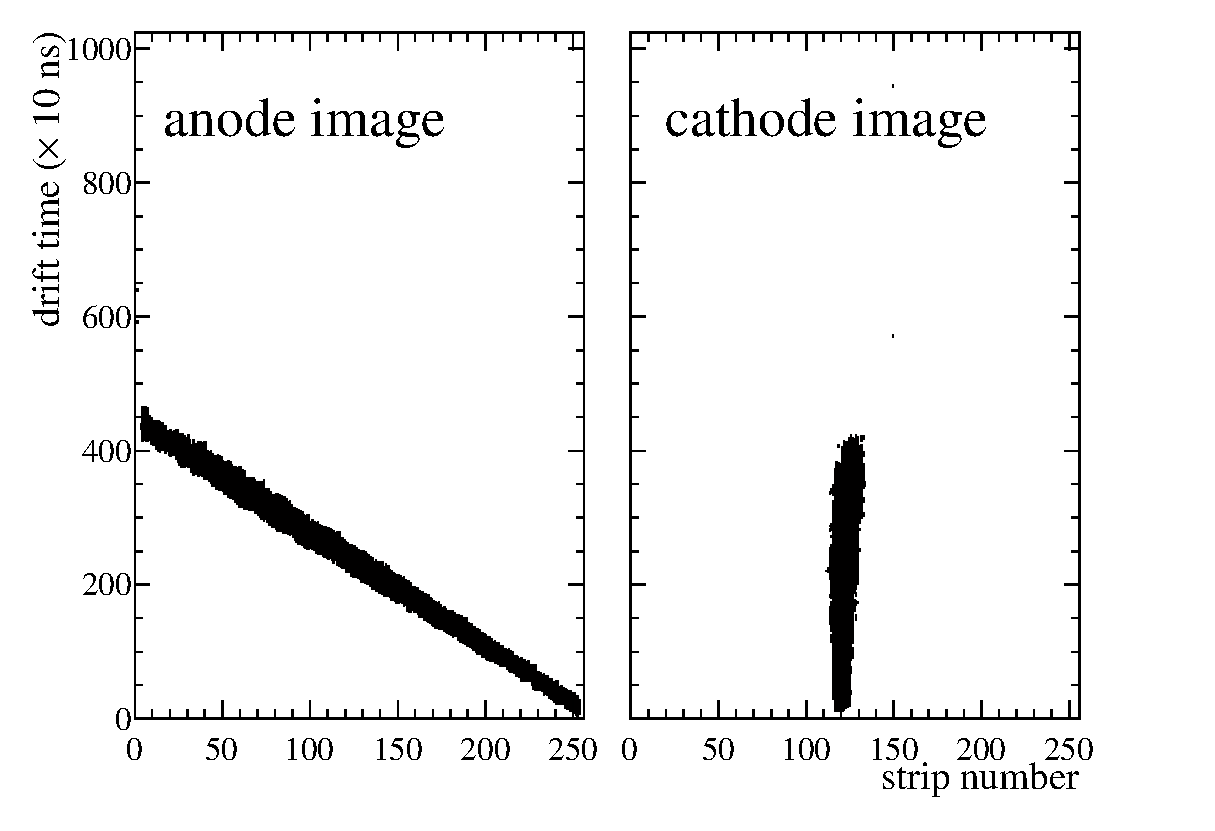
\includegraphics[clip, width=\columnwidth, trim=0 0 50 0]{0207_7.eps}
    \caption{$\alpha$線源によるトラック.}
  \end{subfigure}
  \caption{\MethaneHydro の場合.}
  \label{fig::track_comp_ch4_h2}
\end{figure}

\begin{figure}
  \centering
  \begin{subfigure}{0.48\columnwidth}
    \centering
    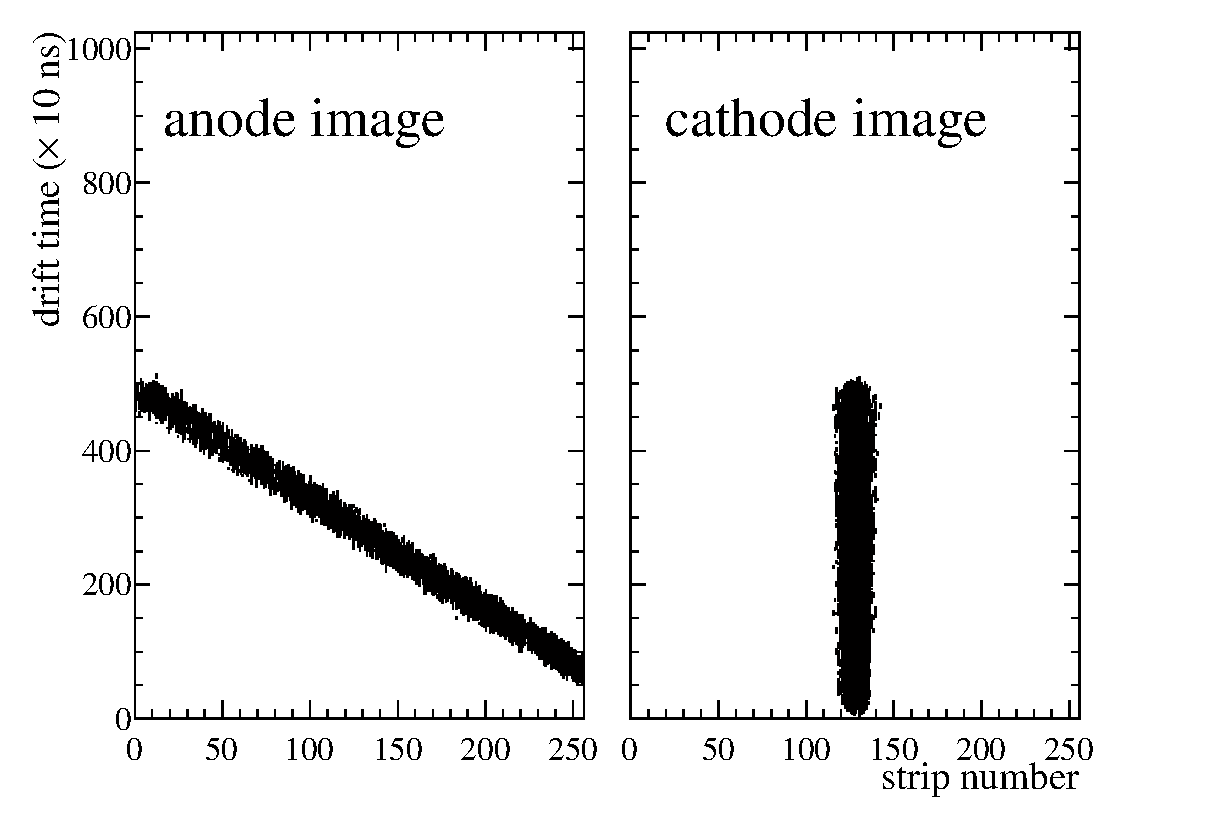
\includegraphics[clip, width=\columnwidth, trim=0 0 50 0]{CH4_4_He_6_0.eps}
    \caption{シミュレーションによるトラック.}
  \end{subfigure}
  \begin{subfigure}{0.48\columnwidth}
    \centering
    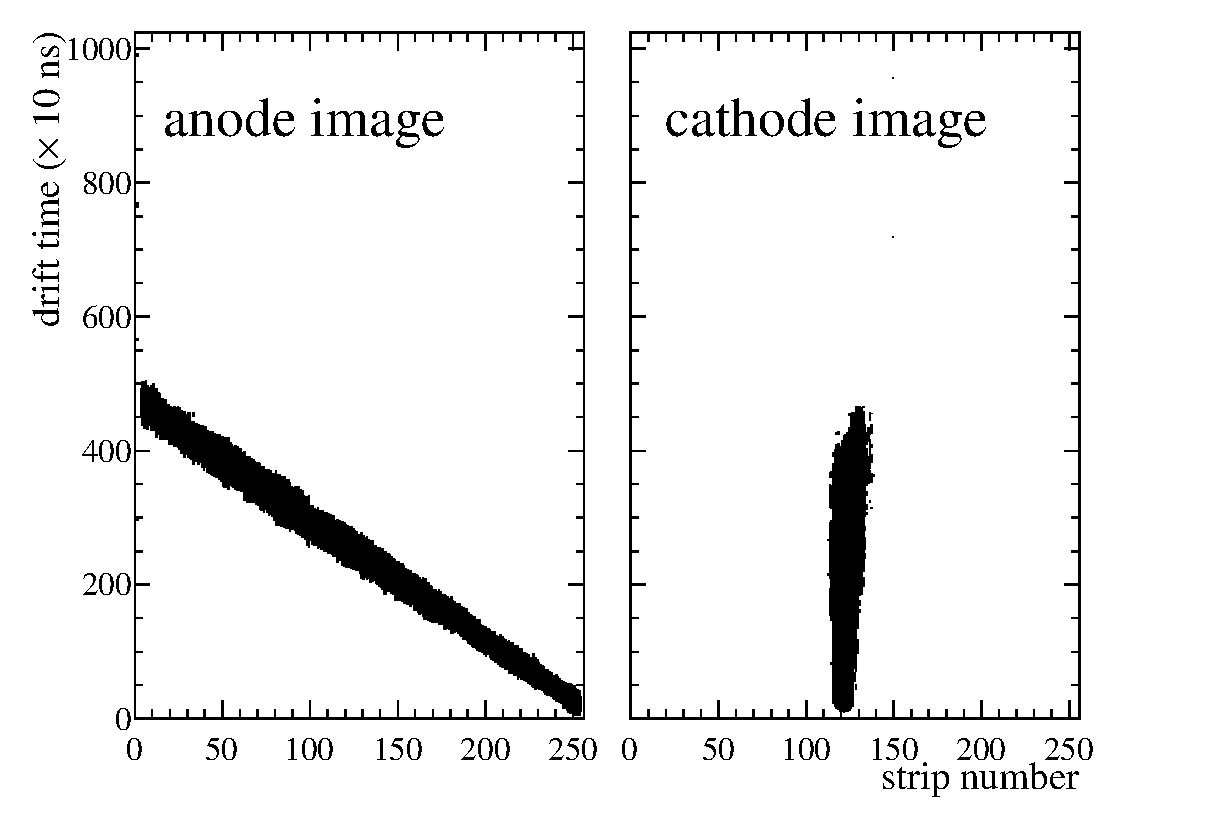
\includegraphics[clip, width=\columnwidth, trim=0 0 50 0]{0163_3.eps}
    \caption{$\alpha$線源によるトラック.}
  \end{subfigure}
  \caption{\MethaneHerium の場合.}
  \label{fig::track_comp_ch4_he}
\end{figure}

\begin{figure}
  \centering
  \begin{subfigure}{0.48\columnwidth}
    \centering
    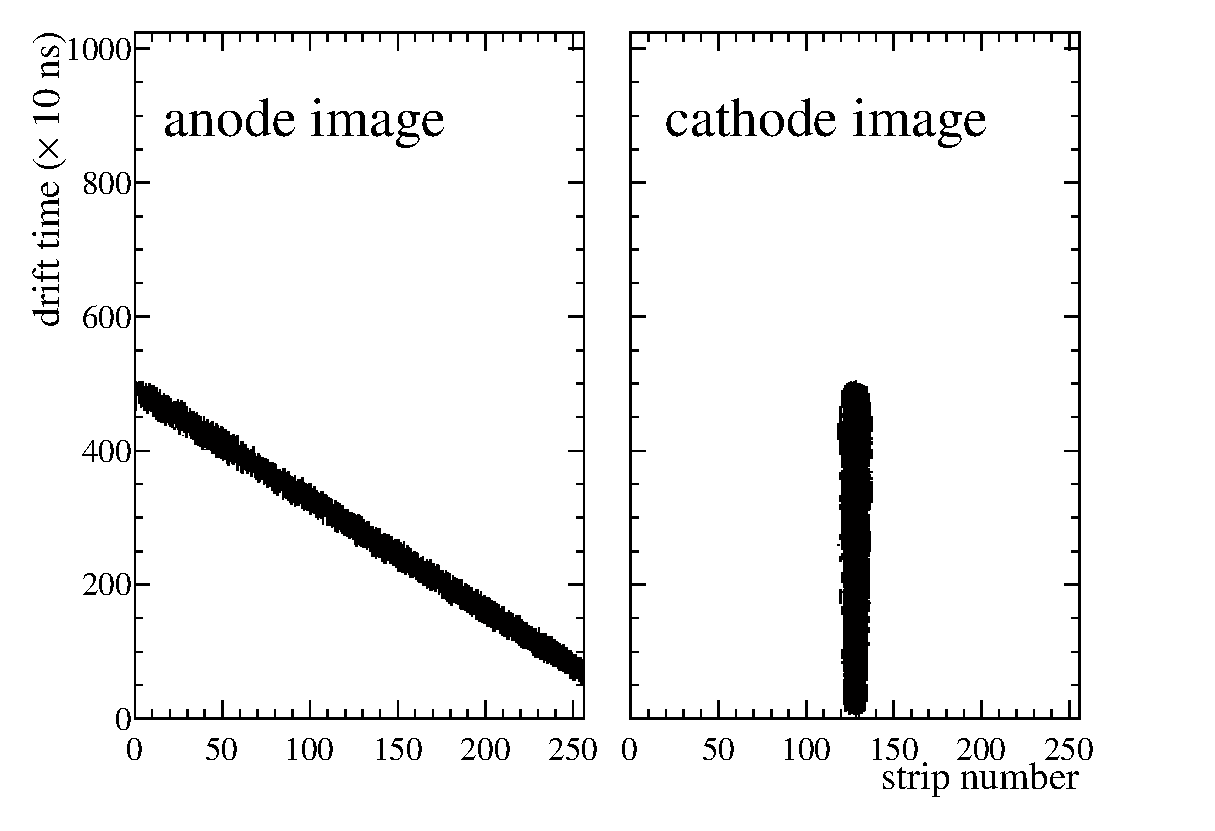
\includegraphics[clip, width=\columnwidth, trim=0 0 50 0]{iC4H10_1_H2_9_0.eps}
    \caption{シミュレーションによるトラック.}
  \end{subfigure}
  \begin{subfigure}{0.48\columnwidth}
    \centering
    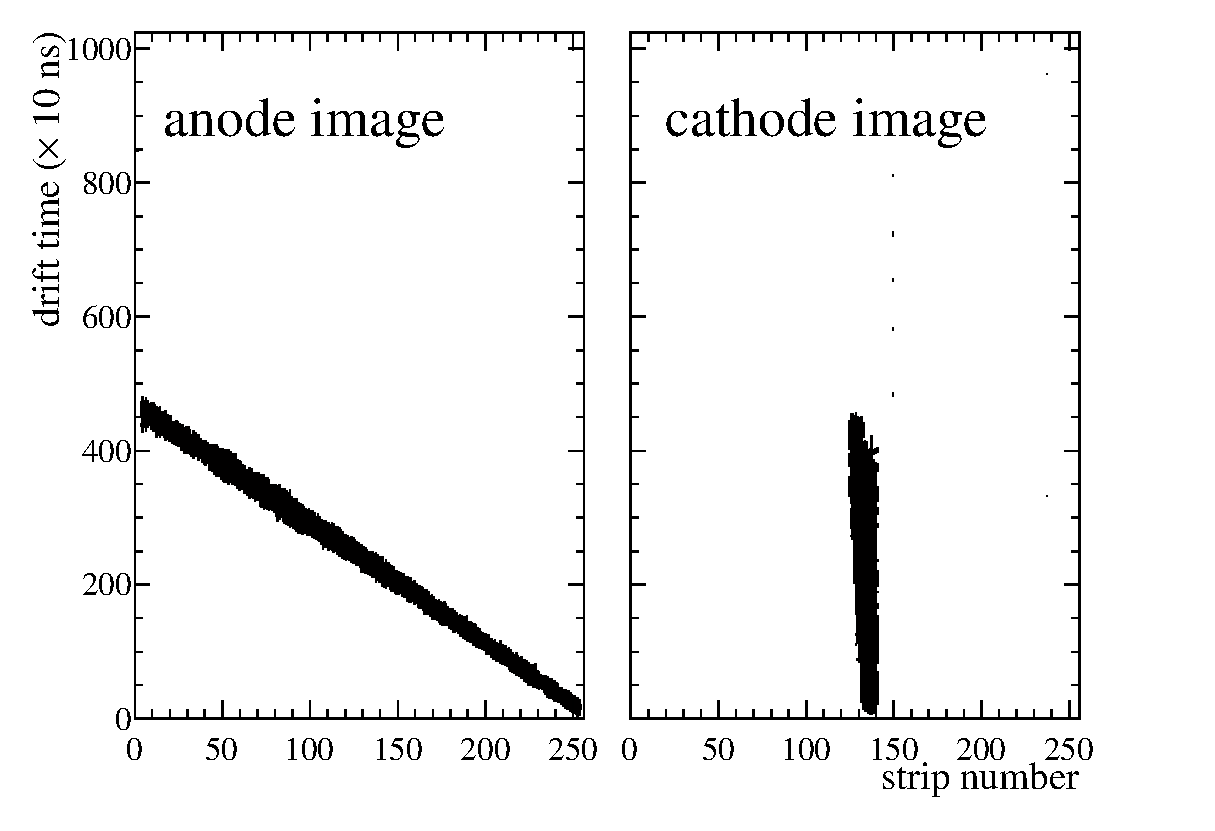
\includegraphics[clip, width=\columnwidth, trim=0 0 50 0]{0210_14.eps}
    \caption{$\alpha$線源によるトラック.}
  \end{subfigure}
  \caption{\isoButaneHydro の場合.}
  \label{fig::track_comp_ic4h10_h2}
\end{figure}

\begin{figure}
  \centering
  \begin{subfigure}{0.48\columnwidth}
    \centering
    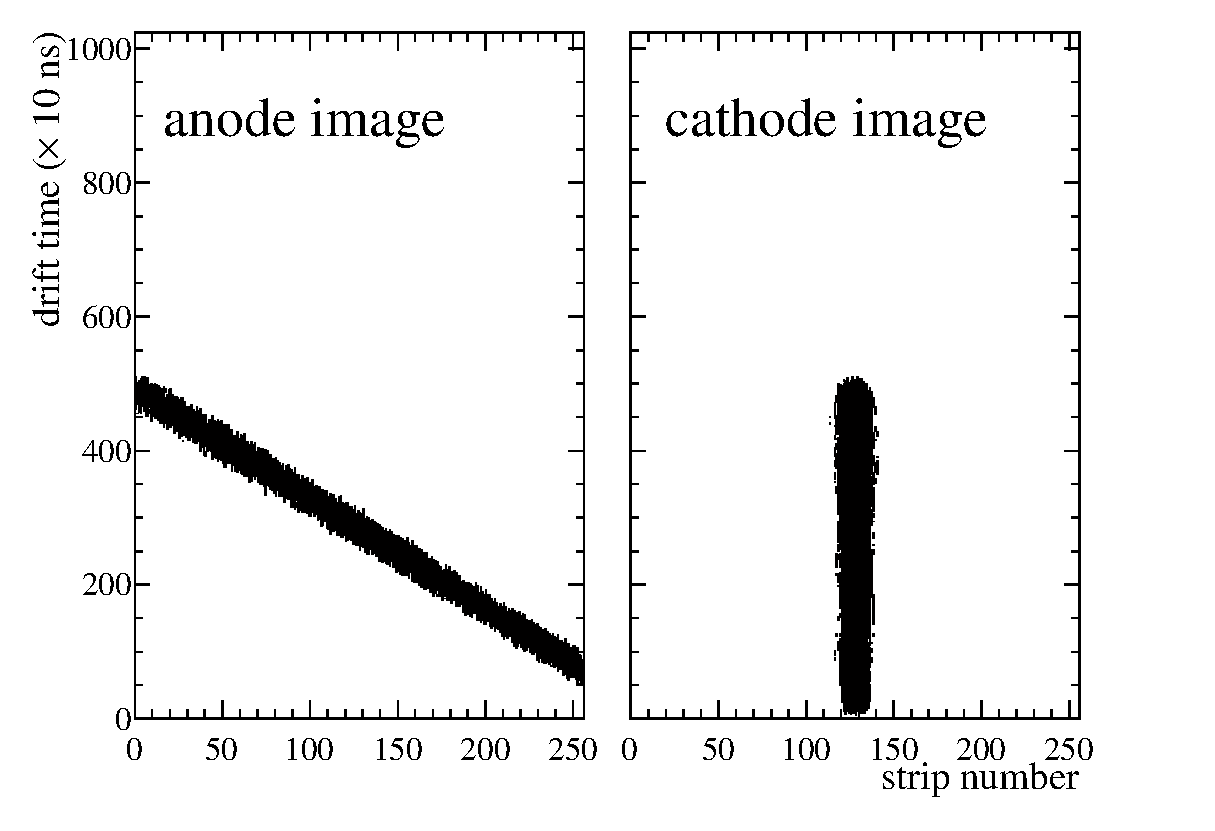
\includegraphics[clip, width=\columnwidth, trim=0 0 50 0]{iC4H10_1_He_9_0.eps}
    \caption{シミュレーションによるトラック.}
  \end{subfigure}
  \begin{subfigure}{0.48\columnwidth}
    \centering
    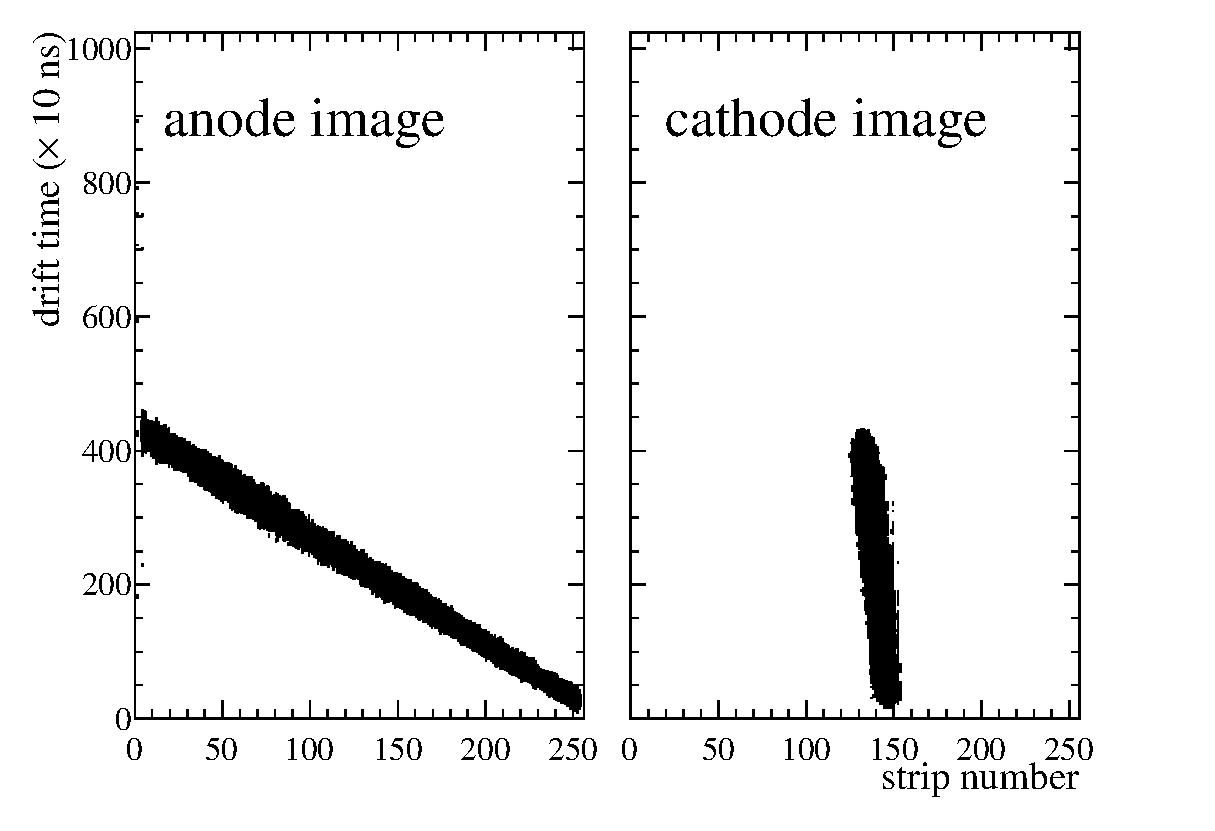
\includegraphics[clip, width=\columnwidth, trim=0 0 50 0]{0176_1.eps}
    \caption{$\alpha$線源によるトラック.}
  \end{subfigure}
  \caption{\isoButaneHerium の場合.}
  \label{fig::track_comp_ic4h10_he}
\end{figure}

\section{トリプルアルファ反応のシミュレーション}
\label{sec::triple_alpha_simulation}
$\alpha$線源のトラックを再現することができたので,
同じ設定で${}^{12}{\rm C}({\rm n},{\rm n}')3\alpha$のシミュレーションを行う.
このシミュレーションでは以下のように3つの$\alpha$粒子を生成した.
\begin{enumerate}
\item
  ${}^{12}{\rm C}$が\SI{14}{\mega\electronvolt}の中性子との散乱によりHoyle状態に励起させる.
  この際,重心系で一様な散乱角で散乱させる.
\item
  Hoyle状態の${}^{12}{\rm C}$を$\alpha$粒子と${}^{8}{\rm Be}$に位相空間で一様に崩壊させる.
\item
  崩壊してできた${}^{8}{\rm Be}$を2つの$\alpha$粒子に位相空間で一様に崩壊させる.
\end{enumerate}
このようにして生成した3つの$\alpha$粒子を元にトラックを生成する.
トラックの生成方法は前節で述べた通りである.
生成したトラックを図\ref{fig::three_alpha_ch4}, \ref{fig::three_alpha_ch4_h2}, \ref{fig::three_alpha_ch4_he},
\ref{fig::three_alpha_ic4h10_h2}, \ref{fig::three_alpha_ic4h10_he}に示す.
ここでは,3つのトラックを確認できたイベントを選んで示した.
\begin{figure}
  \centering
  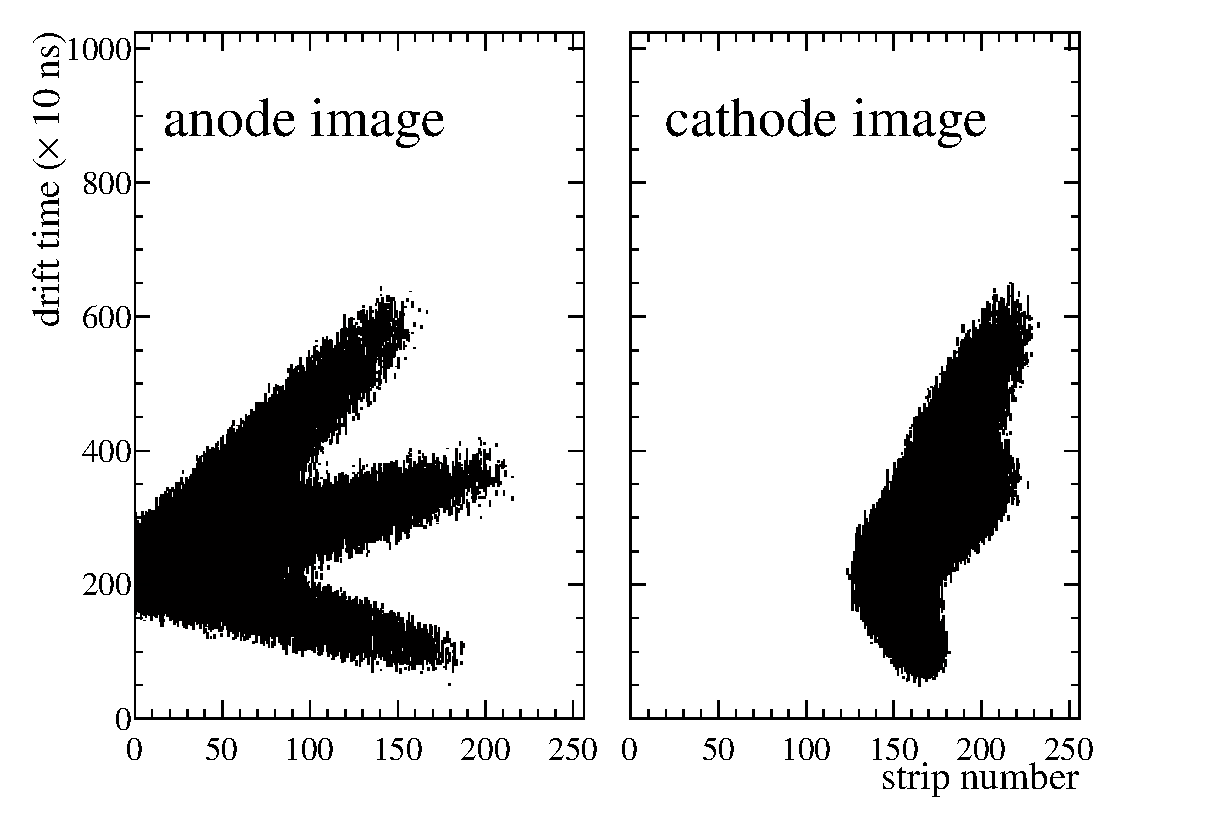
\includegraphics[clip, width=0.8\columnwidth]{10020_7.eps}
  \caption{\Methane の場合.}
  \label{fig::three_alpha_ch4}
\end{figure}

\begin{figure}
  \centering
  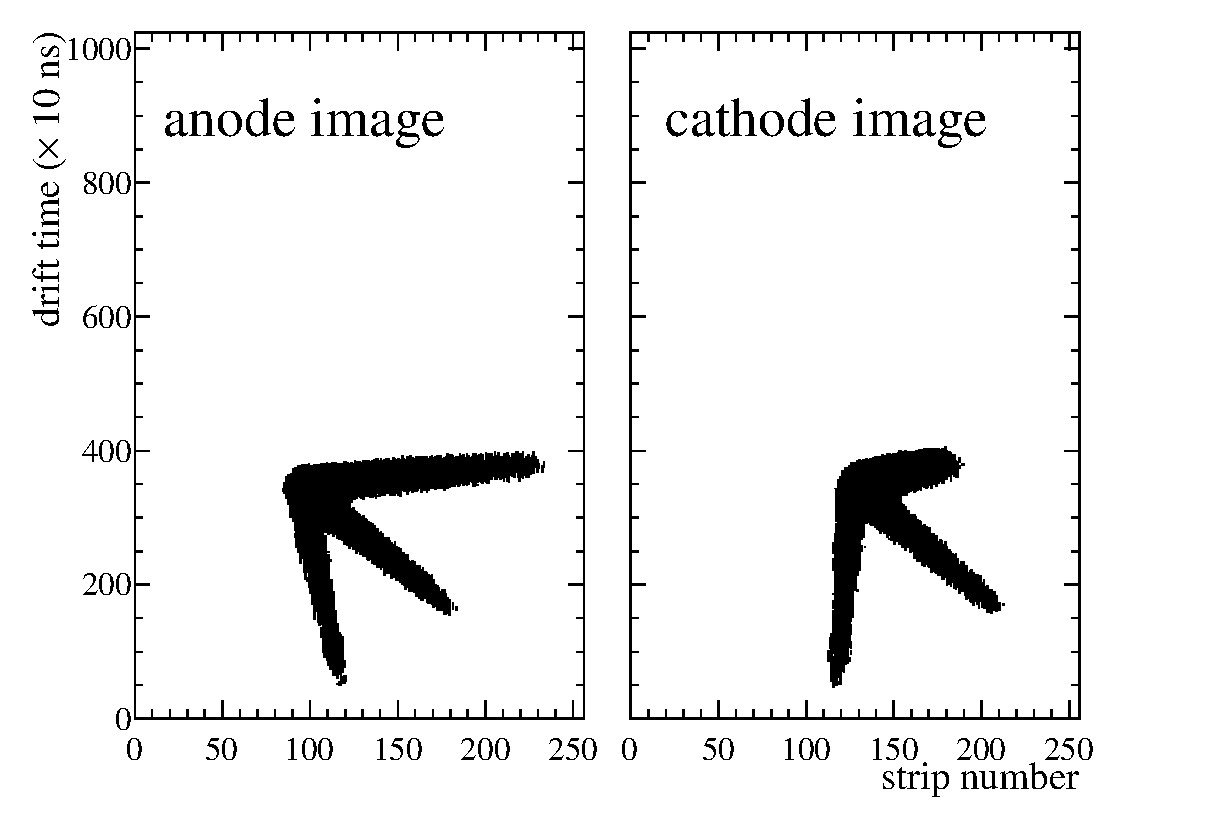
\includegraphics[clip, width=0.8\columnwidth]{10022_15.eps}
  \caption{\MethaneHydro の場合.}
  \label{fig::three_alpha_ch4_h2}
\end{figure}

\begin{figure}
  \centering
  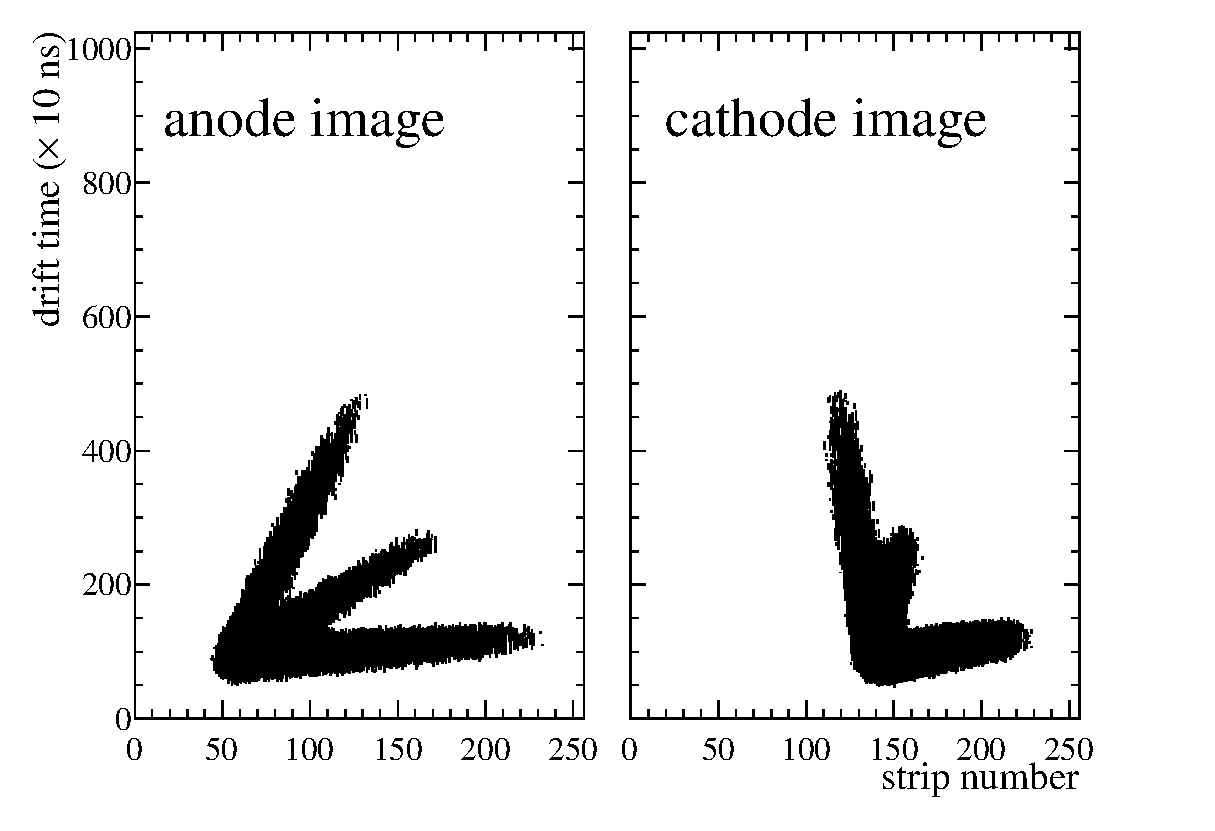
\includegraphics[clip, width=0.8\columnwidth]{10021_5.eps}
  \caption{\MethaneHerium の場合.}
  \label{fig::three_alpha_ch4_he}
\end{figure}

\begin{figure}
  \centering
  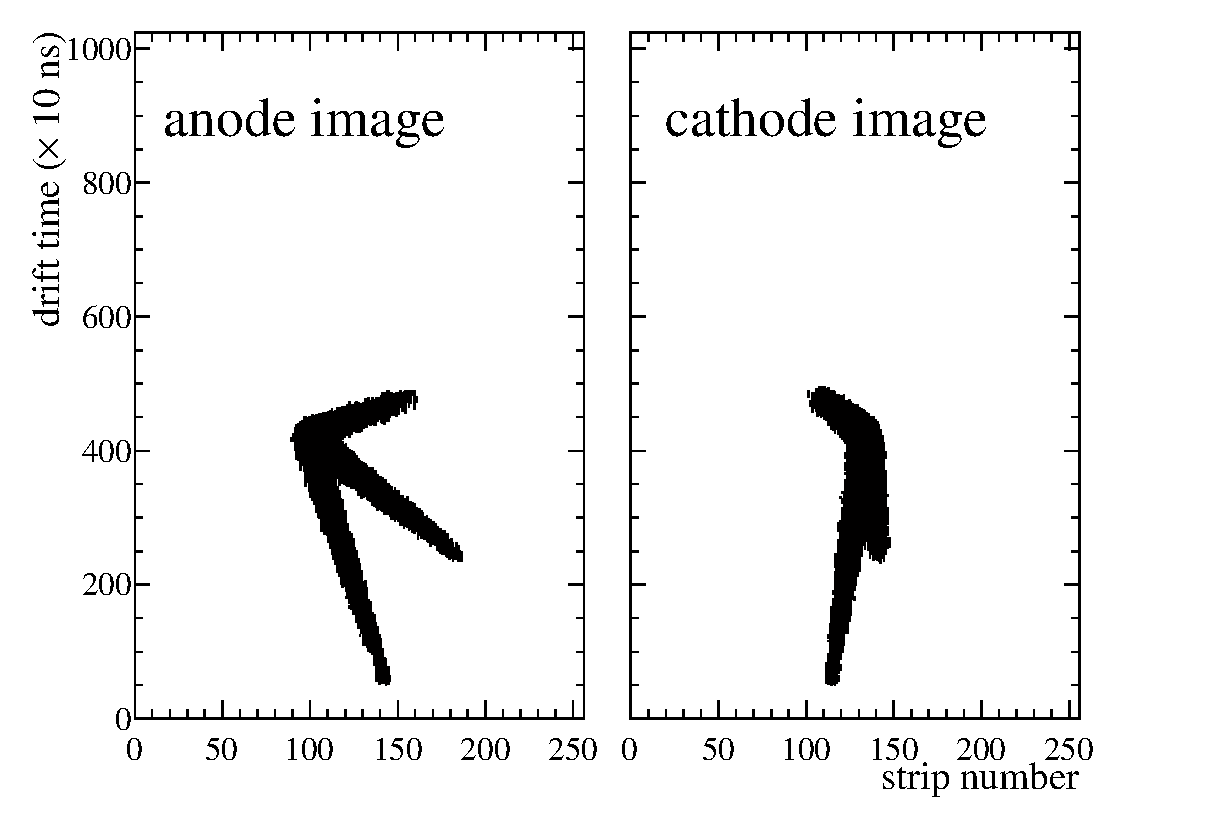
\includegraphics[clip, width=0.8\columnwidth]{10024_9.eps}
  \caption{\isoButaneHydro の場合.}
  \label{fig::three_alpha_ic4h10_h2}
\end{figure}

\begin{figure}
  \centering
  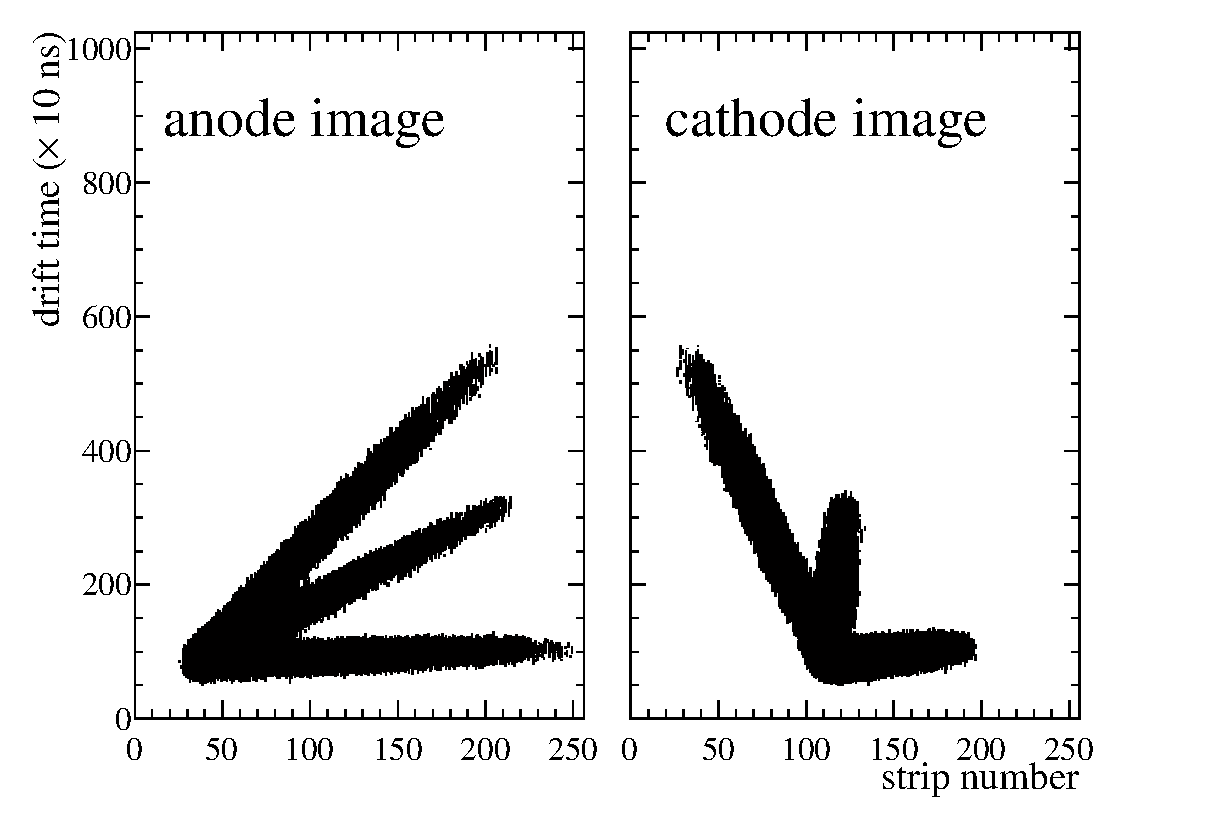
\includegraphics[clip, width=0.8\columnwidth]{10023_0.eps}
  \caption{\isoButaneHerium の場合.}
  \label{fig::three_alpha_ic4h10_he}
\end{figure}

\end{document}
